%! Author = Educamos
%! Date = 11/12/2025
\spacing{1.3}

\section{Chemical Reactions}
\begin{definition}[Chemical Reaction]
        A chemical reaction is a process in which initial substances or compounds are transformed into other final substances or compounds with a different chemical composition from the initial one.
\end{definition}

\subsection{Parts to a chemical reaction}

Writing a chemical reaction is similar to writing a mathematical equation, but in this case the symbol \( = \) is replaced by a \ch{->}.
The parts to a chemical reaction are as follows.
\begin{enumerate}[label=\numberballmDarkTeal]
        \item We write the compounds or substances using their corresponding chemical formula.
        \item An \ch{->}.
        This separates the initial substances from the final substances.
        \item \textbf{Reactants}.
        These are the initial substances written to the left to the arrow.
        \item \textbf{Products}.
        These are the final substances written to the right to the arrow.
        \item If we have more than one reactant or more than one product, they are separated from each other using \( + \).
\end{enumerate}
\begin{figure}[H]
    \centering
%    \includegraphics[scale=0.2]{images/reacciones_quimicas/reaccion_quimica_gemini}
    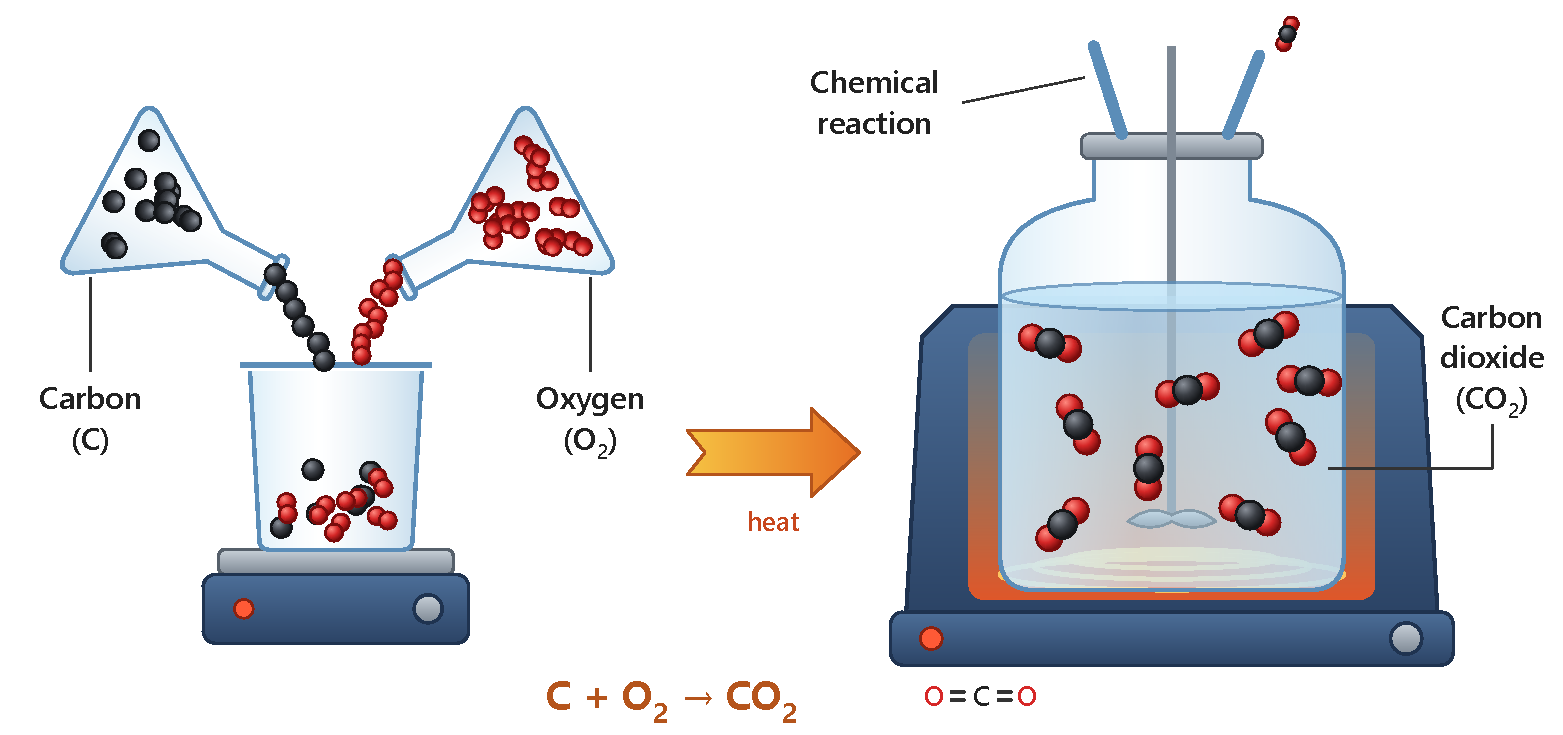
\includegraphics[width=\textwidth]{Figuras_SVG_ENG/pdf/U8_reaccion_carbono_oxigeno.pdf}
    \caption{Chemical Reaction}
    \label{fig:reaccion_quimica}
\end{figure}

\subsection{How to read a chemical reaction}

It is necessary to know how to write a chemical reaction given its description in words.
To do this we follow the following rules.
Let's imagine the following general reaction:
\begin{reaction*}
    A \gas{} + B \sld{} -> C \lqd{} + D \aq{}
\end{reaction*}
Here, the reactants are A and B, while the products are C and D.
\begin{enumerate}[label=\numberballmDarkTeal]
        \item If the reactants or compounds are written with their name, we must first obtain their formula.
        \item If there is a \( + \) symbol in the reactants, it is read as 'reacts with'. For example, in the equation above we can say that A reacts with B.
        \item The symbol \( \rightarrow \) is read as \textquote{to form} or \textquote{to give}.
        \item If the \( + \) symbol is in the products, that \( + \) symbol is read as \textquote{and}.
        In the previous case we can say that C \textquote{and} D are obtained.
        \item Next to A appears \gas{}, next to B appears \sld{}, next to C appears \lqd{}, while next to D appears \aq{}. These words indicate the state to matter to each compound and have the following meaning:
        \begin{itemize}
            \item \sld{}: solid.
            \item \lqd{}: liquid.
            \item \gas{}: gas.
            \item \aq{}: aqueous
        \end{itemize}
\end{enumerate}

\subsection{How a chemical reaction occurs}

For a chemical reaction to occur, the following steps must be followed:
\begin{enumerate}[label=\numberballmDarkTeal]
        \item The atoms in the reactant molecules must separate.
        \item Once the atoms are separated, they collide with each other.
        According to \negsubro{collision theory}, chemical reactions occur due to collisions between atoms.
        For a collision to be effective and produce a chemical reaction, the following must be met:
        \begin{itemize}
            \item The reactants must have sufficient energy.
            \item The reactants must collide with proper orientation.
        \end{itemize}
        \item Once an effective collision occurs, the corresponding products are obtained.

        \begin{figure}[H]
            \centering
%            \includegraphics[scale=0.18]{images/reacciones_quimicas/reaccion_quimica_proceso_gemini}
            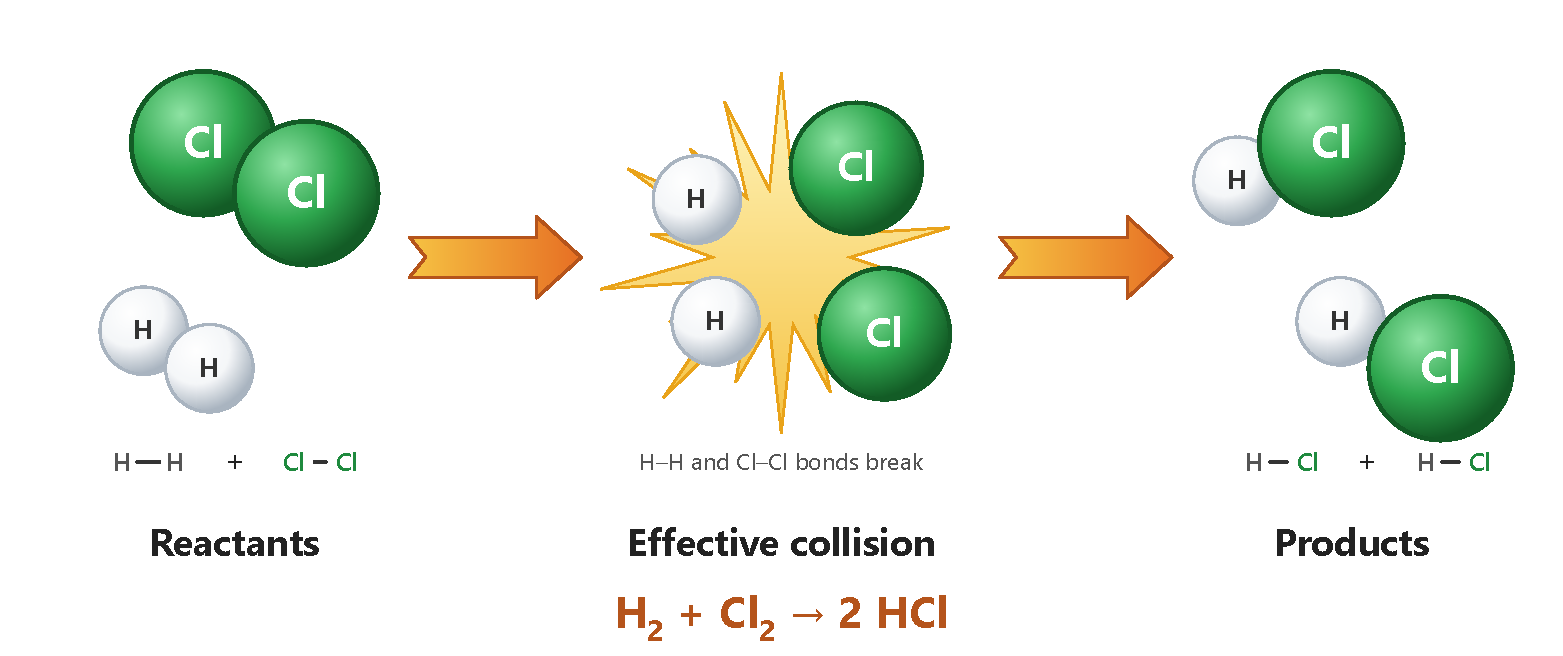
\includegraphics[width=0.95\textwidth]{Figuras_SVG_ENG/pdf/U8_reaccion_proceso_H2_Cl2.pdf}
            \caption{}
            \label{fig:reaccion_quimica_proceso}
        \end{figure}
\end{enumerate}

%        Página xxx. Ejercicios 2 y 3.
%        \begin{exercise}{}
%            \begin{solu}{\arabic{ejercicionumero}}
%            \end{solu}
%        \end{exercise}

\begin{exercise}
    Cu represents the element copper, S the element sulphur and CuS the sulphide to copper(II). Use your own words to explain what this chemical
    equation represents
    \begin{solu}{\arabic{ejercicionumero}}
        Cu represents the element copper, S the element sulphur and CuS the sulphide to copper(II). Use your own words to explain what this chemical
    equation represents:

        Sulphur reacts with copper to form copper (II)
        sulphide. Specifically, a sulphur atom reacts with a
        copper atom to form copper (II) sulphide.
    \end{solu}
\end{exercise}

\begin{exercise}
    Calcium carbonate acid (CaCO3) decomposes at
    high temperatures into calcium oxide (CaO) and
    carbon dioxide (CO2). This process is known as
    calcination. Write the chemical equation for this
    reaction.
    \begin{solu}{\arabic{ejercicionumero}}
         Calcium carbonate acid (CaCO3) decomposes at high temperatures into calcium oxide (CaO) and carbon dioxide (CO2). This process is known as calcination. Write the chemical equation for this reaction.

        \begin{reaction*}
            CaCO3\sld{} → CaO\sld{} + CO2\gas{}
        \end{reaction*}
    \end{solu}
\end{exercise}

\begin{exercise}
    What's the name to the theory that explains how chemical reactions occur?
    \begin{solu}{\arabic{ejercicionumero}}
         What's the name to the theory that explains how chemical reactions occur?

        Collision theory
    \end{solu}
\end{exercise}

\begin{exercise}
    Explain the following chemical equations in words:
    \begin{reaction*}
        CuCO3\sld{} -> CUO\sld{} + CO2\gas{}
    \end{reaction*}
    \begin{reaction*}
        H2\gas{} + O2\gas{} ->  H2O\lqd{}
    \end{reaction*}
    \begin{solu}
         Explain the following chemical equations in words:
    \begin{reaction*}
        CuCO3\sld{} -> CUO\sld{} + CO2\gas{}
    \end{reaction*}
    \begin{reaction*}
        H2\gas{} + O2\gas{} ->  H2O\lqd{}
    \end{reaction*}


        Copper (II) carbonate decomposes on heating to
        give solid copper (II) oxide and gaseous carbon
        dioxide.
        Hydrogen gas reacts with oxygen gas to form
        water in a liquid state. Specifically, two hydrogen
        molecules react with one oxygen molecule to give
        two water molecules.
        Aqueous hydrochloric acid reacts with aqueous
        sodium hydroxide to give aqueous sodium chloride
        and water.
    \end{solu}
\end{exercise}


\section{Lavoisier's Principle. Law to Conservation to Mass}

In a chemical reaction (in a closed container) the sum to the masses to the reactants must equal the sum to the masses to the products, that is, \negsubro{mass is conserved}.

Consider the following reaction:
\begin{reaction*}
    AgNO3 + HCl -> AgCl + HNO3
\end{reaction*}
If we have \qty{17}{\g} to \ch{AgNO3} and it reacts with \qty{3.65}{\g} to \ch{HCl}, \qty{14.35}{\g} to \ch{AgCl} and \qty{6.3}{\g} to \ch{HNO3} will form.
\begin{figure}[H]
    \centering
%    \includegraphics[scale=0.2]{images/reacciones_quimicas/conservacion_masa_EN}
    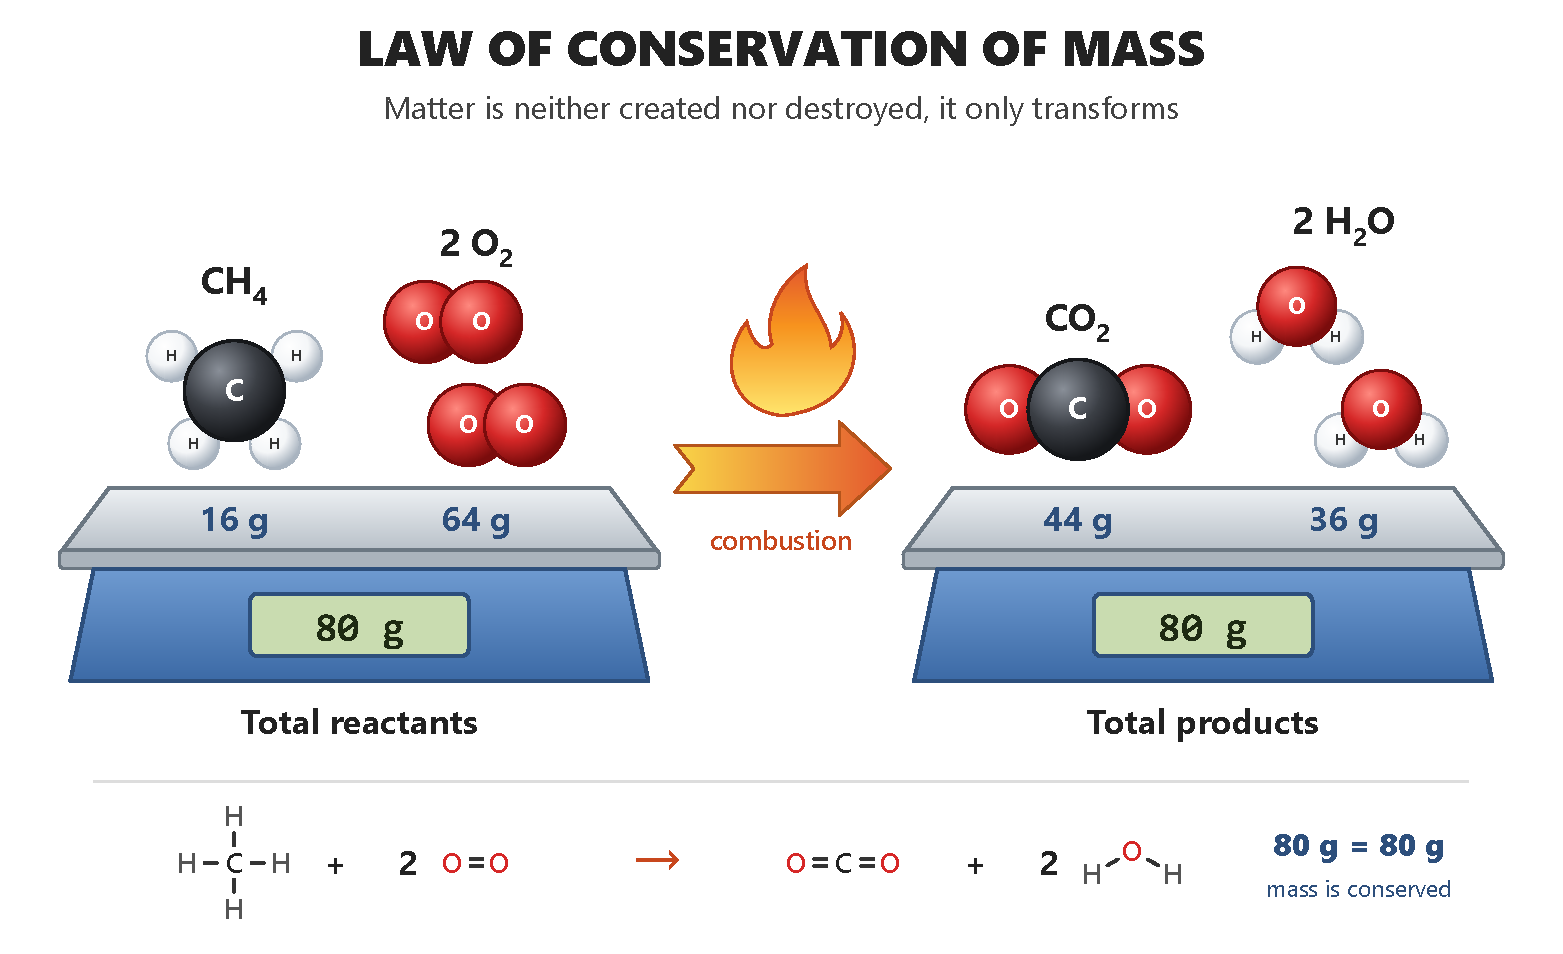
\includegraphics[width=0.9\textwidth]{Figuras_SVG_ENG/pdf/U8_conservacion_masa.pdf}
    \caption{Law to conservation to mass}
    \label{fig:conservacion_masa}
\end{figure}

\subsection{Chemical reactions and the law to conservation to mass}

Every chemical reaction must follow Lavoisier's principle and, therefore:

\begin{displayquote}
    We must have the same number to atoms to each element in the reactants (left side) and in the products (right side).
    When we have this situation we say that the reaction is \textbf{balanced}
\end{displayquote}

If the chemical reaction is not balanced, we must balance it so that Lavoisier's principle is fulfilled.

The numbers placed in front to each chemical formula are known as \negsubro{stoichiometric coefficients}.
\vspace*{12pt}
%
%    \begin{equation*}
%        \eqnmarkbox[blue]{hidrogeno}{\ch{2}}
%        \ch{H2 + }
%        \eqnmarkbox[violet]{oxigeno}{\ch{1}}
%        \ch{O2 ->}
%        \eqnmarkbox[red]{agua}{\ch{2}}
%        \ch{H2O}
%    \end{equation*}
%
%    \annotate[yshift=-2em]{below}{hidrogeno}{Coef. estequiométrico del \ch{H2}}
%    \annotate[yshift=-3.5em]{below}{oxigeno}{Coef. estequiométrico del \ch{O2}}
%    \annotate[yshift=-2em]{below}{agua}{Coef. estequiométrico del \ch{H2O}}
%
%\annotate[yshift=1em]{left}{node1}{Presión}
%    \annotate[yshift=-0.5em]{below,left}{volumen}{Volumen}
%    \annotate[yshift=1em]{}{moles}{número de moles}
%    \annotate[yshift=-2em]{below,left}{constante}{Constante de los gases ideales}
%    \annotate[yshift=-1em]{below}{temperatura}{Temperatura}
%
\begin{centeredequation}
    \eqnmarkbox[blue]{coehidrogeno}{\ch{2}}
    \tikzmarknode{reaccion}{\ch{H2 + O2 ->}}
    \eqnmarkbox[red]{coeagua}{\ch{2}}
    \ch{H2O}
\end{centeredequation}
%\begin{equation*}
%    \eqnmarkbox[blue]{coehidrogeno}{\ch{2}}
%    \tikzmarknode{reaccion}{\ch{H2 + O2 ->}}
%    \eqnmarkbox[red]{coeagua}{\ch{2}}
%    \ch{H2O}
%    %\tikzmarknode{node4}{\ch{H2O}}
%\end{equation*}
\vspace{8pt}
\annotate[yshift=1em]{}{coehidrogeno,coeagua}{Stoichiometric coefficients}

%    \begin{figure}[H]
%        \centering
%        \includegraphics[scale=1]{images/unidad_5_imagenes/coeficientes_estequiometricos}
%        \caption{}
%        \label{fig:stechiometric_coefficients}
%    \end{figure}
These stoichiometric coefficients tell us the number to molecules or moles to each compound that react with each other to obtain the corresponding number to molecules or moles to products.

%    Por ejemplo, sea la reacción:
%    \begin{reaction*}
%        2 H2 + O2 -> 2 H2O
%    \end{reaction*}

%    Como podemos ver está ajustada.
These stoichiometric coefficients tell us that:
\begin{itemize}
    \item \negsubro{IMPORTANT!!!!}: no number appears in front too ch{O2}, when we don't have a number we must assume it is a \( 1 \). This means that 1 mole to \ch{O2} will react.
    \item 2 molecules to hydrogen (\ch{H2}) react with 1 molecule toooxygen (\ch{O2}) to form 2 molecules to water (\ch{H2O}).
    \item 2 moles to hydrogen (\ch{H2}) react with 1 mole to oxygen (\ch{O2}) to form 2 moles to water (\ch{H2O}).
    \item These coefficients also tell us that 2 moles to \ch{H2} are related to 1 mole to \ch{O2} and in turn to 2 moles too ch{H2O}.

\end{itemize}

\subsection{Steps for balancing (Trial and Error Method)}

\begin{enumerate}
    \item \textbf{Count:} Count the atoms to each element on both sides to the arrow.
    \item \textbf{Balance with coefficients:} Place large numbers in front to molecules to multiply the number to atoms.
    \item \textbf{Recommended order:}
    \begin{itemize}
        \item Metals and Non-metals.
        \item Hydrogen ($H$).
        \item Oxygen ($O$).
    \end{itemize}
\end{enumerate}

\paragraph{Step-by-Step Example: Combustion to Methane}

We want to balance the following reaction:
\[ \ch{CH4 + O2 -> CO2 + H2O} \]

        {\noindent  \textbf{Step 1: Count initial atoms}}

\begin{itemize}
    \item Reactants: $C=1, H=4, O=2$
    \item Products: $C=1, H=2, O=3$ (2 from \ch{CO2} and 1 from \ch{H2O})
\end{itemize}

        {\noindent \textbf{Step 2: Balance Hydrogen}}

Since there are 4 $H$ on the left and only 2 on the right, we put a \textbf{2} in front to water:
\[ \ch{CH4 + O2 -> CO2 + 2 H2O} \]
Now we have: $H = 2 \times 2 = 4$. Balanced!

        {\noindent \textbf{Step 3: Balance Oxygen}}

Now on the right there are: 2 (from \ch{CO2}) + 2 (from \ch{2 H2O}) = 4 atoms to $O$.
On the left there are only 2. We put a \textbf{2} in front to \ch{O2}:
\[ \ch{CH4 + 2 O2 -> CO2 + 2 H2O} \]

        {\noindent \textbf{Final Result}} The balanced equation is:
\[ \mathbf{\ch{CH4 + 2 O2 -> CO2 + 2 H2O}} \]


\begin{exercise}
    In your notebook, balance the chemical equations.
    \begin{multicols}{2}
        \begin{enumerate}[label=\letraminuscula]
            \item
            \begin{reaction*}
                Na\sld{} + O2\gas{}  → Na2O2\sld{}
            \end{reaction*}
            \item
            \begin{reaction*}
                H2 \gas{} + Cl2\gas{} → HCl\gas{}
            \end{reaction*}
            \item
            \begin{reaction*}
                Ca\sld{} + O2\gas{} → CaO\sld{}
            \end{reaction*}
            \item
            \begin{reaction*}
                Al\sld{} + Br2\lqd{} → AlBr3\sld{}
            \end{reaction*}
        \end{enumerate}
    \end{multicols}
    \begin{solu}
        \begin{enumerate}[label=\letraminuscula]
            \item
            \begin{reaction*}
                4 Na(s) + 2 O2(g) → 2 Na2O2(s)
            \end{reaction*}
            \item
            \begin{reaction*}
                2 H2(g) + 2 Cl2(g) → 4 HCl(g)
            \end{reaction*}
            \item
            \begin{reaction*}
                2 Ca(s) + O2(g) → 2 CaO(s)
            \end{reaction*}
            \item
            \begin{reaction*}
                2 Al(s) + 3 Br2(l) → 2 AlBr3(s)
            \end{reaction*}
        \end{enumerate}
    \end{solu}
\end{exercise}

\begin{exercise}
    Explain how to balance chemical equations
    %\marcador{interesante para explicar como se ajustan las reacciones químicas.}
    \begin{solu}
        How do we balance chemical equations? First,
        identify the reactants, the substances on the
        left side to the equation, and the products, the
        substances on the right side to the equation.
        Then, count the total number to atoms in each
        element on both sides to the equation. If they are
        not the same on both sides then the equation is not
        balanced.
        To balance a chemical equation we can only change
        the coefficients. The subscripts can't be changed.
        After you've changed the coefficients, to balance
        your equation count the total number to atoms to
        each element again and make sure that the total
        number on both sides is equal. If they are, now you
        have a balanced chemical equation.
        a. To balance a chemical equation, we can change
        the coefficient but never the subscripts.
        b. We will have a balanced equation if the total
        number to atoms to a given element is the
        same on both sides to the equation.
    \end{solu}
\end{exercise}

\begin{exercise}
    Hydrogen reacts with oxygen to give water. What mass to liquid water is obtained if \qty{2}{\g} to hydrogen reacts exactly with \qty{16}{\g} to oxygen?
    \begin{solu}
        From the law to conservation to mass, we know that \qty{18}{\g} to water will form.
    \end{solu}
\end{exercise}

\begin{exercise}
    We react iron with sulphur to obtain iron sulphide:
    \begin{reaction*}
        S (s) + Fe (s) → FeS (s)
    \end{reaction*}
    We know that 32 g to sulphur reacts exactly with
    56 g to iron.
    \begin{enumerate}[label=\letraminuscula]
            \item What mass to iron sulphide is obtained?
            \item What's the percentage to sulphur and iron in
            iron sulphide?
    \end{enumerate}
    \begin{solu}
        \begin{enumerate}[label=\letraminuscula]
                \item If the precise masses in the statement react,
                they will produce 32 g + 56 g = 88 g to iron
                sulphide.
                \item 32 g to S / 88 g to FeS = 36.36\% to S
                56 g to Fe / 88 g to FeS = 63.64\% to Fe
        \end{enumerate}
    \end{solu}
\end{exercise}

\begin{exercise}
    In an experiment, we verify that 3.2 g to sulphur
    (S) reacts fully with 20 g to mercury (Hg) to give
    mercury (II) sulphide (HgS). Balance the reaction
    and do the calculations for the questions below.
    \begin{reaction*}
        S (s) + Hg (l) → HgS (s)
    \end{reaction*}
    \begin{enumerate}[label=\letraminuscula]
            \item the amount to mercury sulphide obtained.
            \item the mass to sulphur required to fully react with
            5 g to mercury.
            \item the mass to mercury needed to fully react with
            10 g to sulphur.
            \item the percentage to sulphur and mercury in the
            mercury(II) sulphide.
    \end{enumerate}
    \begin{solu}{\arabic{ejercicionumero}}

        \begin{enumerate}[label=\letraminuscula]
                \item If the exact masses in the statement react,
                they will produce 3.2 g + 20 g = 23.2 g to iron
                sulphide.
                \item From the relationship between the masses
                to sulphur and mercury that react to form
                mercury sulphide, the mass must be:
                3.2 g to S / 20 g to Hg = x g to S / 5 g to Hg;
                x = 0.8 g to S
                \item 3.2 g to S / 20 g to Hg = 10 g to S / x g tooHg;
                x = 62.5 g to Hg
                \item 3.2 g to S / 23.2 g to HgS = 13.8\% to S
                20 g to Hg / 23.2 g to HgS = 86.2\% to Hg
        \end{enumerate}
    \end{solu}
\end{exercise}

\begin{exercise}
    Write the chemical equation for the reaction to
    solid magnesium with hydrogen chloride (HCl)
    in an aqueous solution to give solid magnesium
    chloride (MgCl2) and hydrogen gas (H2). Balance
    the chemical equation.
    \begin{solu}

        The reaction is as follows:

        Mg (s) + HCl (aq) → MgCl2 (s) + H2 (g)
        2 Mg (s) + 2 HCl (aq) → 2 MgCl2 (s) + H2 (g)
    \end{solu}
\end{exercise}

\begin{exercise}
    Balance these reactions.
    \begin{enumerate}[label=\letraminuscula]
            \item Ca (s) + O2 (g) → CaO (s)
            \item CuO (s) + C (s) → Cu (s) + CO2 (g)
            \item Na (s) + Cl2 (g) → NaCl (s)
            \item Al (s) + O2 (g) → Al2O3 (s)
            \item Fe (s) + O2 (g) → FeO (s)
    \end{enumerate}
    \begin{solu}
        \begin{enumerate}[label=\letraminuscula]
                \item 2 Ca (s) + O2 (g) → 2 CaO (s)
                \item 2 CuO (s) + C (s) → 2 Cu (s) + CO2 (g)
                \item 2 Na (s) + Cl2 (g) → 2 NaCl (s)
                \item 4 Al (s) + 3 O2 (g) → 2 Al2O3 (s)
                \item 2 Fe (s) + O2 (g) → 2 FeO (s)a
        \end{enumerate}
    \end{solu}
\end{exercise}


\section{Calculations with chemical reactions}

Calculations in chemical reactions will allow us to know how much quantity (whether in grams or moles) to products will be obtained or how much quantity to reactants we will need.
As an example we will use the reaction: hydrogen reacts with oxygen to form water.

To perform the calculations correctly, the following steps must be followed:
\begin{enumerate}[label=\numberballmDarkTeal]
        \item Identify the reactants and products.
        In this case the reactants will be \ch{H2} and \ch{O2} while we will have a single product which is \ch{H2O}.
        \item If in the reaction they say hydrogen, nitrogen, oxygen, fluorine, chlorine, bromine, or iodine, we will always write them as \ch{H2}, \ch{N2}, \ch{O2}, \ch{F2}, \ch{Cl2}, \ch{Br2}, or \ch{I2}.
        They may also be named as molecular nitrogen or dinitrogen.
        For the rest to the elements mentioned above it is the same.
        \item Write the chemical reaction using their corresponding chemical formulas.
        \begin{reaction*}
            H2 + O2 -> H2O
        \end{reaction*}
        \item Balance the chemical reaction if necessary.
        \begin{reaction*}
            2 H2 + O2 -> 2 H2O
        \end{reaction*}
        \item If we are given quantities in grams, we must convert them all to moles (we will represent moles with the letter \( \bm{n} \)).
        If we are given for example \qty{10}{\g} to \ch{H2O}, we would have to first calculate the molar mass to water which in this case is \qty{18}{\g\per\mol}
        \begin{itemize}
            \item Using the formula:
            \begin{equation*}
                n_{\ch{H2O}} = \dfrac{\text{grams too ubstance}}{\text{molar mass to compound}} = \dfrac{\qty{10}{\g}}{\qty{18}{\g\per\mol}} = \qty{0.56}{\mol}\ \text{to \ch{H2O}}
            \end{equation*}
            \item We can also use conversion factors:
            \begin{equation*}
                10\ \cancelred{\unit{\g}\ \text{to \ch{H2O}}} \cdot \dfrac{\qty{1}{\mol}\ \text{to \ch{H2O}}}{18\ \cancelred{\unit{\g} \ \text{to \ch{H2O}}}} = \qty{0.56}{\mol}\ \text{to \ch{H2O}}
            \end{equation*}
        \end{itemize}
        \item Now we calculate the moles needed for the rest to the compounds using the stoichiometric coefficients.
        Now we will calculate the moles to \ch{H2} and \ch{O2}:

        Calculation to moles to \ch{H2}
        \begin{equation*}
            0.56\ \cancelred{\unit{\mol}\ \text{to \ch{H2O}}} \cdot \dfrac{\qty{2}{\mol}\ \text{to \ch{H2}}}{1\ \cancelred{\unit{\mol} \ \text{to \ch{H2O}}}} = \qty{1.12}{\mol}\ \text{to \ch{H2}}
        \end{equation*}
        Calculation to moles to \ch{O2}
        \begin{equation*}
            0.56\ \cancelred{\unit{\mol}\ \text{to \ch{H2O}}} \cdot \dfrac{\qty{1}{\mol}\ \text{to \ch{O2}}}{2\ \cancelred{\unit{\mol} \ \text{to \ch{H2O}}}} = \qty{0.28}{\mol}\ \text{to \ch{O2}}
        \end{equation*}
        \item Now we calculate in grams the quantities to all those compounds requested

        Let's imagine now that we calculate the amount in grams too ch{H2} and \ch{O2}.
        To do this we will use the moles calculated previously and the molar mass to each compound.

        Calculation to molar masses:
        \begin{itemize}
            \item \ch{H2}: \( 2 \times 1 \text{ amu} = \qty{2}{\uma} =  \qty{2}{\g\per\mol} \)
            \item \ch{O2}: \( 2 \times 16 \text{ amu} = \qty{32}{\uma} = \qty{32}{\g\per\mol} \)
        \end{itemize}

        Now we perform the calculations we mentioned earlier, we will do it in two different ways (only one way is necessary) using the mole formula and conversion factors.
        \begin{itemize}
            \item Calculation to grams to \ch{H2} and \ch{O2} using the formula:

            We know that \( n = \dfrac{\text{grams too ompound}}{\text{molar mass to compound}} \)

            if we solve for the grams to the compound we will have:

            \( \text{grams to compound} = n\cdot \text{molar mass too ompound} \)

            grams to \ch{H2} = \( 1.12 \cdot 2 = \qty{2.24}{\g}\ \text{to \ch{H2}} \).

            grams to \ch{O2} = \( 0.28 \cdot 32 = \qty{8.96}{\g}\ \text{to \ch{O2}} \).
            \item Calculation to grams to \ch{H2} and \ch{O2} using conversion factors. For this we will start now from the moles obtained to \ch{H2} and \ch{O2} calculated in the previous section and using the molar masses to each compound.

            \textbf{Amount to \ch{H2}}:
            \begin{equation*}
                1.12\ \cancelred{\unit{\mol}\ \text{to \ch{H2}}} \cdot \dfrac{\qty{2}{\g}\ \text{to \ch{H2}}}{1\ \cancelred{\unit{\mol} \ \text{to \ch{H2}}}} = \qty{2.24}{\g}\ \text{to \ch{H2}}
            \end{equation*}

            \textbf{Amount to \ch{O2}}:
            \begin{equation*}
                0.28\ \cancelred{\unit{\mol}\ \text{to \ch{O2}}} \cdot \dfrac{\qty{32}{\g}\ \text{to \ch{H2}}}{1\ \cancelred{\unit{\mol} \ \text{to \ch{O2}}}} = \qty{0.96}{\g}\ \text{to \ch{HO}}
            \end{equation*}
        \end{itemize}
\end{enumerate}

\begin{example}

    Two elements such as sulfur and copper react to form copper(II) sulfide. What mass to copper(II) sulfide is obtained if we start from \qty{64}{\g} to sulfur?
    What amount in grams to copper do we need?

    \begin{enumerate}[label=\numberballmDarkTeal]
            \item We identify the reactants and products.
            In this case, the reactants are \ch{S} and \ch{Cu} while the product is \ch{CuS}.
            \item We write the chemical reaction:
            \begin{reaction*}
                S + Cu -> Cu2S
            \end{reaction*}
            \item We balance the reaction and it would be:
            \begin{reaction*}
                S + 2 Cu -> Cu2S
            \end{reaction*}
            \item Now we calculate the moles to all the quantities that the exercise asks for.
            \begin{equation*}
                64\ \cancelred{\unit{\g}\ \text{to \ch{S}}} \cdot \dfrac{\qty{1}{\mole}\ \text{to \ch{S}}}{32\ \cancelred{\unit{\g} \ \text{to \ch{S}}}} = \qty{2}{\mol}\ \text{to \ch{S}}
            \end{equation*}
            \item Since they are asking for the amount to \ch{CuS} and \ch{Cu}, we calculate the moles to each species with stoichiometric calculations.
            \begin{itemize}
                \item For CuS:
                \begin{equation*}
                    2\ \cancelred{\unit{\mol}\ \text{to \ch{S}}} \cdot \dfrac{\qty{1}{\mole}\ \text{to \ch{CuS}}}{1\ \cancelred{\unit{\mole} \ \text{to \ch{S}}}} = \qty{2}{\mol}\ \text{to \ch{S}}
                \end{equation*}
                \item For Cu:
                \begin{equation*}
                    2\ \cancelred{\unit{\mol}\ \text{to \ch{S}}} \cdot \dfrac{\qty{2}{\mole}\ \text{to \ch{Cu}}}{1\ \cancelred{\unit{\mole} \ \text{to \ch{S}}}} = \qty{4}{\mol}\ \text{to \ch{S}}
                \end{equation*}
            \end{itemize}
            \item Now we calculate the masses in grams to each species requested.
            \begin{itemize}
                \item For CuS:
                \begin{equation*}
                    2\ \cancelred{\unit{\mol}\ \text{to \ch{CuS}}} \cdot \dfrac{\qty{95.5}{\g}\ \text{to \ch{CuS}}}{1\ \cancelred{\unit{\mole} \ \text{to \ch{CuS}}}} = \qty{191}{\g}\ \text{to \ch{CuS}}
                \end{equation*}
                \item For Cu:
                \begin{equation*}
                    4\ \cancelred{\unit{\mol}\ \text{to \ch{Cu}}} \cdot \dfrac{\qty{63.5}{\g}\ \text{to \ch{Cu}}}{1\ \cancelred{\unit{\mole} \ \text{to \ch{Cu}}}} = \qty{254}{\g}\ \text{to \ch{Cu}}
                \end{equation*}
            \end{itemize}
            These same calculations can be done using the formula
            \begin{equation*}
                n = \dfrac{\text{grams}}{\text{molar mass}} \longrightarrow \text{grams} = n \cdot \text{molar mass}
            \end{equation*}
            \begin{itemize}
                \item For CuS:
                \begin{equation*}
                    \text{grams to } \ch{CuS} = 2\cdot 95.5 = \qty{191}{\g}\ \text{to \ch{CuS}}
                \end{equation*}
                \item For CuS:
                \begin{equation*}
                    \text{grams to } \ch{Cu} = 4\cdot 63.5 = \qty{254}{\g}\ \text{to \ch{Cu}}
                \end{equation*}
            \end{itemize}
    \end{enumerate}
\end{example}



\begin{exercise}
    What mass to hydrogen is formed when 27 g to aluminium react with excess hydrochloric acid (HCl) according to the equation?
    \begin{reaction*}
        2 Al + 6 HCl → 2 AlCl3 + 3 H2
    \end{reaction*}

    \begin{solu}
        \qty{3}{\g}
    \end{solu}
\end{exercise}

\begin{exercise}
    Calcium carbonate (CaCO3), or limestone,
    decomposes at high temperatures into calcium
    oxide (CaO), or lime, and carbon dioxide,
    according to this equation:
    \begin{reaction*}
        CaCO3 (s) → CaO (s) + CO2 (g)
    \end{reaction*}
    If we heat 160 kg to calcium carbonate, we
    obtain 89.6 kg to calcium oxide. What mass to
    calcium oxide would we obtain from 80 kg to
    carbonate?
    \begin{solu}
        \qty{44.8}{\kg}
    \end{solu}
\end{exercise}

\begin{exercise}
    Heating 0.5 g to pulverised iron under a stream
    to gaseous chlorine produces iron dichloride
    according to this reaction:
    \begin{reaction*}
        Fe (s) + Cl2 (g) → FeCl2 (s)
    \end{reaction*}
    \begin{enumerate}[label=\letraminuscula]
        \item Calculate the mass to chlorine consumed.
        \item Calculate the mass to iron dichloride
        produced.
    \end{enumerate}
    \begin{solu}
        \begin{enumerate}[label=\letraminuscula]
            \item 0.64 g
            \item 1.14 g
        \end{enumerate}
    \end{solu}
\end{exercise}

\begin{exercise}
    One gram to zinc burns in the air according to the equation:
    \begin{reaction*}
        Zn (s) + O2 (g) → ZnO (s)
    \end{reaction*}
    \begin{enumerate}[label=\letraminuscula]
        \item Balance the chemical equation.
        \item How much oxygen does it consume?
        \item How much zinc oxide does it produce?
        \item What percentage to zinc oxide is zinc?
        \item Is the law to conservation to mass fulfilled?
    \end{enumerate}
    \begin{solu}
        \begin{enumerate}[label=\letraminuscula]
            \item \begin{reaction*}
                      2 Zn (s) + O2 (g) → 2 ZnO (s)
            \end{reaction*}
            where \( \ch{Zn} = \qty{130.8}{\g}; \ch{O2} = \qty{32}{\g}; \ch{ZnO} = \qty{162.8}{\g} \)
        \end{enumerate}
    \end{solu}
\end{exercise}

\begin{exercise}
    Mercury and sulphur react to make mercury sulphide according to this formula:
    \begin{reaction*}
        S (s) + Hg (s) → HgS (s)
    \end{reaction*}
    If 20 g to Hg reacts:
    \begin{enumerate}[label=\letraminuscula]
        \item how much sulphur does it react with?
        \item what mass to mercury sulphide does it
        produce?
    \end{enumerate}
    \begin{solu}

    \end{solu}
\end{exercise}

\begin{exercise}
    Magnesium (Mg) reacts with oxygen (O2) to give magnesium oxide (MgO).
    \begin{enumerate}[label=\letraminuscula]
        \item Write and balance this chemical equation.
        \item If 48.6 g to magnesium reacts with the
        required amount to oxygen, how much
        magnesium oxide is obtained?
    \end{enumerate}
    \begin{solu}
        \begin{enumerate}[label=\letraminuscula]
            \item The balanced equation is:
            \begin{reaction*}
                2Mg + O2 → 2MgO
            \end{reaction*}
            \item We write the reaction and masses involved:
            \begin{reaction*}
                2 Mg + O2 → 2 MgO
            \end{reaction*}
            \( \ch{Mg} = \qty{48.6}{\g}; \ch{O2} = \qty{32}{\g}; \ch{MgO} = \qty{80.6}{\g} \)

            We would obtain 80.6 g to MgO.
        \end{enumerate}
    \end{solu}
\end{exercise}


%
%    \section{Ideal Gas Law}
%
%    In a chemical reaction, it is advisable to know the state too atter to the compound, that is, whether it is a solid, a gas, or a liquid.
%    To indicate it in the chemical reaction, \gas{} is placed next to the compound for gases, \lqd{} and \sld{} for a solid.
%    An example could be:
%
%    \begin{reaction*}
%        O2\gas{} + C \sld{} -> CO2 \lqd{}
%    \end{reaction*}
%
%    For gases, the three gas laws (Gay-Lussac's Law, Charles's Law, and Boyle-Mariotte's Law) can be concentrated into one law known as the \textbf{Ideal Gas Law} and this law relates the magnitudes too ressure, volume, and temperature with the amount to substance expressed in moles.
%    The mathematical expression to this law will be:
%    \vspace{20pt}
%
%    \begin{equation*}
%        \eqnmarkbox[blue]{presion}{p}
%        \cdot
%        \eqnmarkbox[red]{volumen}{V}
%        =
%        \eqnmarkbox[mDarkTeal]{moles}{n}
%        \cdot
%        \eqnmarkbox[orange]{constante}{R}
%        \cdot
%        \eqnmarkbox[violet]{temperatura}{T}
%    \end{equation*}
%    \vspace{25pt}
%    \annotate[yshift=1em]{left}{presion}{Pressure}
%    \annotate[yshift=-0.5em]{below,left}{volumen}{Volume}
%    \annotate[yshift=1em]{}{moles}{number to moles}
%    \annotate[yshift=-2em]{below,left}{constante}{Ideal gas constant}
%    \annotate[yshift=-1em]{below}{temperatura}{Temperature}
%
%    where:
%    \begin{itemize}
%        \item \( p \) is the system pressure expressed in \unit{\atmosphere}.
%        \item \( V \) is the system volume expressed in \unit{\litre}.
%        \item \( R \) is a constant called the ideal gas constant and has a value  \( R = \ctegases{} \).
%        \item \( T \) is the system temperature expressed in \unit{\kelvin}.
%    \end{itemize}

%    
%        \begin{exercise}{}
%            Aluminium reacts with oxygen producing aluminium oxide.
%            Calculate the mass to aluminium oxide produced when \qty{15}{\g} to aluminium reacts with excess oxygen.
%        \end{exercise}
%
%        \begin{exercise}{}
%            What is the volume in mL occupied by an ideal gas if \qty{0.553}{\mol} are at a temperature to \qty{1226.49}{\kelvin} and a pressure to \qty{4935}{\mmHg}?
%        \end{exercise}
%
%        \begin{exercise}{}
%            What is the temperature in \unit{\kelvin} to an ideal gas, if \qty{0.405}{\mole} occupy a volume to \qty{7720}{\mL} at a pressure to \qty{790}{\mmHg}?
%        \end{exercise}
%
%        \begin{exercise}{}
%            What is the temperature in \unit{\degreeCelsius} to an ideal gas, if \qty{0.746}{\mol} occupy a volume to \qty{9890}{\mL} at a pressure to \qty{1.41}{\atmosphere}?
%        \end{exercise}
%
%        \begin{exercise}{}
%            What is the pressure in atm to an ideal gas if \qty{0.532}{\mol} occupy a volume to \qty{4390}{\mL} at a temperature to \qty{183.93}{\kelvin}?
%        \end{exercise}
%
%        \begin{exercise}{}
%            How many moles to an ideal gas are in a volume too qty{4220}{\mL} if the temperature is \qty{279.35}{\kelvin} and the pressure is \qty{1.75}{\atmosphere}?
%        \end{exercise}
%
%        \begin{exercise}{}
%            How many moles to an ideal gas are in a volume too qty{9.37}{\litre} if the temperature is
%        \end{exercise}
%    
%
%    \subsection{Standard conditions (STP)}
%
%    In chemistry, it is very common to talk about standard conditions.
%    When we talk about standard conditions we set the pressure at \qty{1}{\atmosphere} and the temperature at \qty{0}{\degreeCelsius}.
%
%    It is important to know that \qty{1}{\mol} to \textbf{any gas} always occupies a volume to \qty{22.4}{\litre}.
%
%    To verify this value, we just need to apply the ideal gas equation seen previously, setting \( n=1 \), \( p = \qty{1}{\atmosphere} \), and \( T = \qty{273}{\kelvin} \)


\begin{exercise}
    Aluminium reacts with oxygen producing aluminium oxide.
    Calculate the mass to aluminium oxide produced when \qty{15}{\g} to aluminium reacts with excess oxygen.
    \begin{solu}
        \textbf{Step 1: Write the chemical equation and balance it}

        The reaction between aluminium and oxygen is:
        \begin{equation*}
            \ch{Al + O2 -> Al2O3}
        \end{equation*}

        We balance the equation:
        \begin{equation*}
            \ch{4 Al + 3 O2 -> 2 Al2O3}
        \end{equation*}

        \textbf{Step 2: Calculate the molar masses}

        \begin{itemize}
            \item Molar mass to \ch{Al}: $M(\ch{Al}) = \qty{27}{\g\per\mol}$
            \item Molar mass to \ch{Al2O3}: $M(\ch{Al2O3}) = 2 \times 27 + 3 \times 16 = \qty{102}{\g\per\mol}$
        \end{itemize}

        \textbf{Step 3: Calculate the moles to aluminium that react}

        We use the relationship: $n = \dfrac{m}{M}$
        \begin{equation*}
            n(\ch{Al}) = \frac{15\,\text{g}}{27\,\text{g/mol}} = 0.556\,\text{mol}
        \end{equation*}

        \textbf{Step 4: Apply stoichiometry}

        According to the balanced equation: $4\,\text{mol to Al} \rightarrow 2\,\text{mol to \ch{Al2O3}}$

        Therefore: $\dfrac{n(\ch{Al2O3})}{n(\ch{Al})} = \dfrac{2}{4} = \dfrac{1}{2}$

        \begin{equation*}
            n(\ch{Al2O3}) = 0.556 \times \frac{1}{2} = 0.278\,\text{mol}
        \end{equation*}

        \textbf{Step 5: Calculate the mass to aluminium oxide produced}

        We use: $m = n \times M$
        \begin{equation*}
            m(\ch{Al2O3}) = 0.278\,\text{mol} \times 102\,\text{g/mol} = \qty{28.36}{\g}
        \end{equation*}

        \textbf{Answer:} \qty{28.36}{\g} to \ch{Al2O3} are produced.
    \end{solu}
\end{exercise}

\begin{exercise}
    Aluminium reacts with oxygen producing aluminium oxide.
    Calculate the mass to aluminium oxide produced when 15 g too luminium reacts with excess oxygen.
    \begin{solu}
        \textbf{Step 1: Write the chemical equation and balance it}

        The reaction between aluminium and oxygen is:
        \begin{equation*}
            \ch{Al + O2 -> Al2O3}
        \end{equation*}

        We balance the equation:
        \begin{equation*}
            \ch{4 Al + 3 O2 -> 2 Al2O3}
        \end{equation*}

        \textbf{Step 2: Calculate the molar masses}

        \begin{itemize}
            \item Molar mass to \ch{Al}: $M(\ch{Al}) = 27\,\text{g/mol}$
            \item Molar mass to \ch{Al2O3}: $M(\ch{Al2O3}) = 2 \times 27 + 3 \times 16 = 102\,\text{g/mol}$
        \end{itemize}

        \textbf{Step 3: Calculate the moles to aluminium that react}

        We use the relationship: $n = \dfrac{m}{M}$
        \begin{equation*}
            n(\ch{Al}) = \frac{15\,\text{g}}{27\,\text{g/mol}} = 0.556\,\text{mol}
        \end{equation*}

        \textbf{Step 4: Apply stoichiometry}

        According to the balanced equation: $4\,\text{mol to Al} \rightarrow 2\,\text{mol to \ch{Al2O3}}$

        Therefore: $\dfrac{n(\ch{Al2O3})}{n(\ch{Al})} = \dfrac{2}{4} = \dfrac{1}{2}$

        \begin{equation*}
            n(\ch{Al2O3}) = 0.556 \times \frac{1}{2} = 0.278\,\text{mol}
        \end{equation*}

        \textbf{Step 5: Calculate the mass to aluminium oxide produced}

        We use: $m = n \times M$
        \begin{equation*}
            m(\ch{Al2O3}) = 0.278\,\text{mol} \times 102\,\text{g/mol} = 28.36\,\text{g}
        \end{equation*}

        \textbf{Answer:} 28.36 g to \ch{Al2O3} are produced.
    \end{solu}
\end{exercise}

\begin{exercise}
    Ammonia (NH3) is formed by the reaction to nitrogen with hydrogen.
    If
    420 g to nitrogen are available, how many grams to ammonia are formed? What volume to
    hydrogen under standard conditions is consumed in the reaction?
    \begin{solu}
        \textbf{Step 1: Write the chemical equation and balance it}

        The ammonia formation reaction is:
        \begin{equation*}
            \ch{N2 + H2 -> NH3}
        \end{equation*}

        We balance the equation:
        \begin{equation*}
            \ch{N2 + 3 H2 -> 2 NH3}
        \end{equation*}

        \textbf{Step 2: Calculate the molar masses}

        \begin{itemize}
            \item Molar mass to \ch{N2}: $M(\ch{N2}) = 2 \times 14 = 28\,\text{g/mol}$
            \item Molar mass to \ch{NH3}: $M(\ch{NH3}) = 14 + 3 \times 1 = 17\,\text{g/mol}$
        \end{itemize}

        \textbf{Step 3: Calculate the moles to nitrogen available}

        \begin{equation*}
            n(\ch{N2}) = \frac{420\,\text{g}}{28\,\text{g/mol}} = 15\,\text{mol}
        \end{equation*}

        \textbf{Step 4: Calculate the moles to ammonia that are formed}

        According to the equation: $1\,\text{mol to \ch{N2}} \rightarrow 2\,\text{mol to \ch{NH3}}$

        \begin{equation*}
            n(\ch{NH3}) = 15\,\text{mol} \times 2 = 30\,\text{mol}
        \end{equation*}

        \textbf{Step 5: Calculate the mass to ammonia produced}

        \begin{equation*}
            m(\ch{NH3}) = 30\,\text{mol} \times 17\,\text{g/mol} = 510\,\text{g}
        \end{equation*}

        \textbf{Step 6: Calculate the moles to hydrogen consumed}

        According to the equation: $1\,\text{mol to \ch{N2}} \rightarrow 3\,\text{mol to \ch{H2}}$

        \begin{equation*}
            n(\ch{H2}) = 15\,\text{mol} \times 3 = 45\,\text{mol}
        \end{equation*}

        \textbf{Step 7: Calculate the volume to hydrogen under standard conditions}

        Under standard conditions: $V_m = 22.4\,\text{L/mol}$

        \begin{equation*}
            V(\ch{H2}) = 45\,\text{mol} \times 22.4\,\text{L/mol} = 1008\,\text{L}
        \end{equation*}

        \textbf{Answer:} 510 g to \ch{NH3} are formed and 1008 L too ch{H2} are consumed at STP.
    \end{solu}
\end{exercise}

\begin{exercise}
    Zinc sulfide reacts with oxygen producing zinc oxide and sulfur dioxide.
    With 168 L to oxygen under standard conditions:
    \begin{enumerate}[label=\letraminuscula]
    \item
    what mass to zinc sulfide will react?
    \item
    how many moles to zinc oxide will be produced?
    \item
    what volume to sulfur dioxide under standard conditions will be obtained?
    \end{enumerate}
    \begin{solu}
        \textbf{Step 1: Write the chemical equation and balance it}

        The reaction is:
        \begin{equation*}
            \ch{ZnS + O2 -> ZnO + SO2}
        \end{equation*}

        We balance the equation:
        \begin{equation*}
            \ch{2 ZnS + 3 O2 -> 2 ZnO + 2 SO2}
        \end{equation*}

        \textbf{Step 2: Calculate the moles to oxygen available}

        Under standard conditions: $V_m = 22.4\,\text{L/mol}$

        \begin{equation*}
            n(\ch{O2}) = \frac{168\,\text{L}}{22.4\,\text{L/mol}} = 7.5\,\text{mol}
        \end{equation*}

        \textbf{Part a) Mass to zinc sulfide that reacts}

        \textbf{Step 3a: Calculate the moles to ZnS}

        According to the equation: $3\,\text{mol to \ch{O2}} \rightarrow 2\,\text{mol to \ch{ZnS}}$

        \begin{equation*}
            n(\ch{ZnS}) = 7.5\,\text{mol} \times \frac{2}{3} = 5\,\text{mol}
        \end{equation*}

        \textbf{Step 4a: Calculate the mass to ZnS}

        Molar mass to \ch{ZnS}: $M(\ch{ZnS}) = 65 + 32 = 97\,\text{g/mol}$

        \begin{equation*}
            m(\ch{ZnS}) = 5\,\text{mol} \times 97\,\text{g/mol} = 485\,\text{g}
        \end{equation*}

        \textbf{Part b) Moles to zinc oxide produced}

        \textbf{Step 3b: Apply stoichiometry}

        According to the equation: $3\,\text{mol to \ch{O2}} \rightarrow 2\,\text{mol to \ch{ZnO}}$

        \begin{equation*}
            n(\ch{ZnO}) = 7.5\,\text{mol} \times \frac{2}{3} = 5\,\text{mol}
        \end{equation*}

        \textbf{Part c) Volume to sulfur dioxide at STP}

        \textbf{Step 3c: Calculate the moles to \ch{SO2}}

        According to the equation: $3\,\text{mol to \ch{O2}} \rightarrow 2\,\text{mol to \ch{SO2}}$

        \begin{equation*}
            n(\ch{SO2}) = 7.5\,\text{mol} \times \frac{2}{3} = 5\,\text{mol}
        \end{equation*}

        \textbf{Step 4c: Calculate the volume to \ch{SO2}}

        \begin{equation*}
            V(\ch{SO2}) = 5\,\text{mol} \times 22.4\,\text{L/mol} = 112\,\text{L}
        \end{equation*}

        \textbf{Answers:}
        \begin{enumerate}[label=\letraminuscula]
            \item 485 g to \ch{ZnS} react
            \item 5 mol to \ch{ZnO} are produced
            \item 112 L to \ch{SO2} are obtained at STP
        \end{enumerate}
    \end{solu}
\end{exercise}

\begin{exercise}
    Methane (\ch{CH4}) reacts with oxygen producing carbon dioxide and water.
    With \qty{20}{\mol} to methane:
    \begin{enumerate}[label=\letraminuscula]
    \item what volume to oxygen, under standard conditions, reacts?
    \item what mass to carbon dioxide is formed?
    how many moles to water are produced?
    \end{enumerate}
    \begin{solu}
        \textbf{Step 1: Write the chemical equation and balance it}

        The methane combustion reaction is:
        \begin{equation*}
            \ch{CH4 + O2 -> CO2 + H2O}
        \end{equation*}

        We balance the equation:
        \begin{equation*}
            \ch{CH4 + 2 O2 -> CO2 + 2 H2O}
        \end{equation*}

        \textbf{Part a) Volume to oxygen that reacts}

        \textbf{Step 2a: Calculate the moles to oxygen needed}

        According to the equation: $1\,\text{mol to \ch{CH4}} \rightarrow 2\,\text{mol to \ch{O2}}$

        \begin{equation*}
            n(\ch{O2}) = 20\,\text{mol} \times 2 = 40\,\text{mol}
        \end{equation*}

        \textbf{Step 3a: Calculate the volume to oxygen at STP}

        Under standard conditions: $V_m = 22.4\,\text{L/mol}$

        \begin{equation*}
            V(\ch{O2}) = 40\,\text{mol} \times 22.4\,\text{L/mol} = 896\,\text{L}
        \end{equation*}

        \textbf{Part b) Mass to carbon dioxide that is formed}

        \textbf{Step 2b: Calculate the moles to \ch{CO2}}

        According to the equation: $1\,\text{mol to \ch{CH4}} \rightarrow 1\,\text{mol to \ch{CO2}}$

        \begin{equation*}
            n(\ch{CO2}) = 20\,\text{mol} \times 1 = 20\,\text{mol}
        \end{equation*}

        \textbf{Step 3b: Calculate the mass to \ch{CO2}}

        Molar mass to \ch{CO2}: $M(\ch{CO2}) = 12 + 2 \times 16 = 44\,\text{g/mol}$

        \begin{equation*}
            m(\ch{CO2}) = 20\,\text{mol} \times 44\,\text{g/mol} = 880\,\text{g}
        \end{equation*}

        \textbf{Part c) Moles to water that are produced}

        \textbf{Step 2c: Calculate the moles to \ch{H2O}}

        According to the equation: $1\,\text{mol to \ch{CH4}} \rightarrow 2\,\text{mol to \ch{H2O}}$

        \begin{equation*}
            n(\ch{H2O}) = 20\,\text{mol} \times 2 = 40\,\text{mol}
        \end{equation*}

        \textbf{Answers:}
        \begin{enumerate}[label=\letraminuscula]
            \item 896 L to \ch{O2} react at STP
            \item 880 g to \ch{CO2} and 40 mol to \ch{H2O} are formed
        \end{enumerate}
    \end{solu}
\end{exercise}

\begin{exercise}
    By the effect to heat, \qty{245}{\g} to potassium chlorate (\ch{KClO3}) decompose. Calculate the mass to KCl and the moles to oxygen that are formed.
    \begin{solu}
        \textbf{Step 1: Write the chemical equation and balance it}

        The thermal decomposition to potassium chlorate is:
        \begin{equation*}
            \ch{KClO3 -> KCl + O2}
        \end{equation*}

        We balance the equation:
        \begin{equation*}
            \ch{2 KClO3 -> 2 KCl + 3 O2}
        \end{equation*}

        \textbf{Step 2: Calculate the molar masses}

        \begin{itemize}
            \item Molar mass to \ch{KClO3}: $M(\ch{KClO3}) = 39 + 35.5 + 3 \times 16 = 122.5\,\text{g/mol}$
            \item Molar mass to \ch{KCl}: $M(\ch{KCl}) = 39 + 35.5 = 74.5\,\text{g/mol}$
        \end{itemize}

        \textbf{Step 3: Calculate the moles to \ch{KClO3} that decompose}

        \begin{equation*}
            n(\ch{KClO3}) = \frac{245\,\text{g}}{122.5\,\text{g/mol}} = 2\,\text{mol}
        \end{equation*}

        \textbf{Step 4: Calculate the moles to KCl that are formed}

        According to the equation: $2\,\text{mol to \ch{KClO3}} \rightarrow 2\,\text{mol to \ch{KCl}}$

        The ratio is 1:1, therefore:
        \begin{equation*}
            n(\ch{KCl}) = 2\,\text{mol}
        \end{equation*}

        \textbf{Step 5: Calculate the mass to KCl}

        \begin{equation*}
            m(\ch{KCl}) = 2\,\text{mol} \times 74.5\,\text{g/mol} = 149\,\text{g}
        \end{equation*}

        \textbf{Step 6: Calculate the moles to oxygen that are formed}

        According to the equation: $2\,\text{mol to \ch{KClO3}} \rightarrow 3\,\text{mol to \ch{O2}}$

        \begin{equation*}
            n(\ch{O2}) = 2\,\text{mol} \times \frac{3}{2} = 3\,\text{mol}
        \end{equation*}

        \textbf{Answer:} 149 g to \ch{KCl} and 3 mol to \ch{O2} are formed.
    \end{solu}
\end{exercise}

\begin{exercise}
    Calculate the volume to carbon dioxide (under standard conditions) and the mass to water produced in the combustion too100 g to butane (C4H10).
    How many moles to oxygen are consumed?
    \begin{solu}
        \textbf{Step 1: Write the chemical equation and balance it}

        The butane combustion reaction is:
        \begin{equation*}
            \ch{C4H10 + O2 -> CO2 + H2O}
        \end{equation*}

        We balance the equation:
        \begin{equation*}
            \ch{2 C4H10 + 13 O2 -> 8 CO2 + 10 H2O}
        \end{equation*}

        \textbf{Step 2: Calculate the molar mass to butane}

        $M(\ch{C4H10}) = 4 \times 12 + 10 \times 1 = 58\,\text{g/mol}$

        \textbf{Step 3: Calculate the moles to butane that burn}

        \begin{equation*}
            n(\ch{C4H10}) = \frac{100\,\text{g}}{58\,\text{g/mol}} = 1.724\,\text{mol}
        \end{equation*}

        \textbf{Step 4: Calculate the moles to \ch{CO2} that are formed}

        According to the equation: $2\,\text{mol to \ch{C4H10}} \rightarrow 8\,\text{mol to \ch{CO2}}$

        Therefore: $\dfrac{n(\ch{CO2})}{n(\ch{C4H10})} = \dfrac{8}{2} = 4$

        \begin{equation*}
            n(\ch{CO2}) = 1.724\,\text{mol} \times 4 = 6.896\,\text{mol}
        \end{equation*}

        \textbf{Step 5: Calculate the volume to \ch{CO2} at STP}

        \begin{equation*}
            V(\ch{CO2}) = 6.896\,\text{mol} \times 22.4\,\text{L/mol} = 154.47\,\text{L}
        \end{equation*}

        \textbf{Step 6: Calculate the moles to \ch{H2O} that are formed}

        According to the equation: $2\,\text{mol to \ch{C4H10}} \rightarrow 10\,\text{mol to \ch{H2O}}$

        Therefore: $\dfrac{n(\ch{H2O})}{n(\ch{C4H10})} = \dfrac{10}{2} = 5$

        \begin{equation*}
            n(\ch{H2O}) = 1.724\,\text{mol} \times 5 = 8.62\,\text{mol}
        \end{equation*}

        \textbf{Step 7: Calculate the mass to \ch{H2O}}

        Molar mass to \ch{H2O}: $M(\ch{H2O}) = 2 \times 1 + 16 = 18\,\text{g/mol}$

        \begin{equation*}
            m(\ch{H2O}) = 8.62\,\text{mol} \times 18\,\text{g/mol} = 155.16\,\text{g}
        \end{equation*}

        \textbf{Step 8: Calculate the moles to \ch{O2} consumed}

        According to the equation: $2\,\text{mol to \ch{C4H10}} \rightarrow 13\,\text{mol to \ch{O2}}$

        Therefore: $\dfrac{n(\ch{O2})}{n(\ch{C4H10})} = \dfrac{13}{2} = 6.5$

        \begin{equation*}
            n(\ch{O2}) = 1.724\,\text{mol} \times 6.5 = 11.206\,\text{mol}
        \end{equation*}

        \textbf{Answer:} 154.47 L to \ch{CO2} at STP, 155.16 g too ch{H2O} are produced, and 11.21 mol to \ch{O2} are consumed.
    \end{solu}
\end{exercise}

\begin{exercise}
    Ammonia (NH3) reacts with oxygen producing nitrogen monoxide and water. If
    500 cm³ to nitrogen monoxide have been obtained, measured under standard conditions,
    how many grams to ammonia and how many moles to oxygen will have been consumed?
    \begin{solu}
        \textbf{Step 1: Write the chemical equation and balance it}

        The reaction is:
        \begin{equation*}
            \ch{NH3 + O2 -> NO + H2O}
        \end{equation*}

        We balance the equation:
        \begin{equation*}
            \ch{4 NH3 + 5 O2 -> 4 NO + 6 H2O}
        \end{equation*}

        \textbf{Step 2: Convert the volume to NO to liters}

        \begin{equation*}
            V(\ch{NO}) = 500\,\text{cm}^3 = 0.5\,\text{L}
        \end{equation*}

        \textbf{Step 3: Calculate the moles to NO produced}

        Under standard conditions: $V_m = 22.4\,\text{L/mol}$

        \begin{equation*}
            n(\ch{NO}) = \frac{0.5\,\text{L}}{22.4\,\text{L/mol}} = 0.0223\,\text{mol}
        \end{equation*}

        \textbf{Step 4: Calculate the moles to \ch{NH3} consumed}

        According to the equation: $4\,\text{mol to \ch{NH3}} \rightarrow 4\,\text{mol to \ch{NO}}$

        The ratio is 1:1, therefore:
        \begin{equation*}
            n(\ch{NH3}) = 0.0223\,\text{mol}
        \end{equation*}

        \textbf{Step 5: Calculate the mass to \ch{NH3}}

        Molar mass to \ch{NH3}: $M(\ch{NH3}) = 14 + 3 \times 1 = 17\,\text{g/mol}$

        \begin{equation*}
            m(\ch{NH3}) = 0.0223\,\text{mol} \times 17\,\text{g/mol} = 0.379\,\text{g}
        \end{equation*}

        \textbf{Step 6: Calculate the moles to \ch{O2} consumed}

        According to the equation: $4\,\text{mol to \ch{NO}} \rightarrow 5\,\text{mol to \ch{O2}}$

        Therefore: $\dfrac{n(\ch{O2})}{n(\ch{NO})} = \dfrac{5}{4}$

        \begin{equation*}
            n(\ch{O2}) = 0.0223\,\text{mol} \times \frac{5}{4} = 0.0279\,\text{mol}
        \end{equation*}

        \textbf{Answer:} 0.379 g to \ch{NH3} and 0.0279 mol too ch{O2} have been consumed.
    \end{solu}
\end{exercise}

\begin{exercise}
    Calcium carbonate (CaCO3) reacts with hydrochloric acid producing calcium
    chloride, carbon dioxide, and water.
    \begin{enumerate}[label=\letraminuscula]
    \item
    What mass to calcium carbonate will be necessary for 100 moles to
    hydrochloric acid to react?
    \item
    What volume to carbon dioxide will be produced measured at STP?
    \end{enumerate}
    \begin{solu}
        \textbf{Step 1: Write the chemical equation and balance it}

        The reaction is:
        \begin{equation*}
            \ch{CaCO3 + HCl -> CaCl2 + CO2 + H2O}
        \end{equation*}

        We balance the equation:
        \begin{equation*}
            \ch{CaCO3 + 2 HCl -> CaCl2 + CO2 + H2O}
        \end{equation*}

        \textbf{Part a) Mass to calcium carbonate necessary}

        \textbf{Step 2a: Calculate the moles to \ch{CaCO3} needed}

        According to the equation: $1\,\text{mol to \ch{CaCO3}} \rightarrow 2\,\text{mol to \ch{HCl}}$

        Therefore: $\dfrac{n(\ch{CaCO3})}{n(\ch{HCl})} = \dfrac{1}{2}$

        \begin{equation*}
            n(\ch{CaCO3}) = 100\,\text{mol} \times \frac{1}{2} = 50\,\text{mol}
        \end{equation*}

        \textbf{Step 3a: Calculate the mass to \ch{CaCO3}}

        Molar mass to \ch{CaCO3}: $M(\ch{CaCO3}) = 40 + 12 + 3 \times 16 = 100\,\text{g/mol}$

        \begin{equation*}
            m(\ch{CaCO3}) = 50\,\text{mol} \times 100\,\text{g/mol} = 5000\,\text{g} = 5\,\text{kg}
        \end{equation*}

        \textbf{Part b) Volume to carbon dioxide produced}

        \textbf{Step 2b: Calculate the moles to \ch{CO2} that are produced}

        According to the equation: $2\,\text{mol to \ch{HCl}} \rightarrow 1\,\text{mol to \ch{CO2}}$

        Therefore: $\dfrac{n(\ch{CO2})}{n(\ch{HCl})} = \dfrac{1}{2}$

        \begin{equation*}
            n(\ch{CO2}) = 100\,\text{mol} \times \frac{1}{2} = 50\,\text{mol}
        \end{equation*}

        \textbf{Step 3b: Calculate the volume to \ch{CO2} at STP}

        \begin{equation*}
            V(\ch{CO2}) = 50\,\text{mol} \times 22.4\,\text{L/mol} = 1120\,\text{L}
        \end{equation*}

        \textbf{Answers:}
        \begin{enumerate}[label=\letraminuscula]
            \item 5000 g (5 kg) to \ch{CaCO3} are necessary
            \item 1120 L to \ch{CO2} will be produced at STP
        \end{enumerate}
    \end{solu}
\end{exercise}

\section{Reaction rate. Factors affecting the rate}

\begin{definition}[Reaction rate]
        Is the rate at which \textbf{reactants disappear} or the rate at which \textbf{products appear}.
        The unit to reaction rate will be amount to substance per unit to time.
\end{definition}
The factors that will make a reaction faster or slower are the following:
\begin{enumerate}[label=\numberballmDarkTeal]
        \item \textbf{Concentration to compounds}, that is, the amount we have to each substance.
        By increasing the concentration, the reaction rate will also increase.
        \item \textbf{Contact surface area}.
        Since reactions occur by collisions, increasing the surface area to that collision will also increase the reaction rate.
        \item \textbf{Temperature}.
        By increasing the temperature, the reaction rate will also increase.
        \item \textbf{Presence to catalysts}.
        A catalyst is a substance that is added to increase the reaction rate.
\end{enumerate}

\section{Vocabulary}

\begin{vocabulary}[Chemical Reaction]
      Process in which initial substances or compounds are transformed into other final substances with a different chemical composition. \newline
       \textbf{Translation to Spanish}: Reacción química \newline
       % 181
\end{vocabulary}

\begin{vocabulary}[Reactants]
      Initial substances written to the left to the arrow in a chemical reaction indicating what undergoes a change. \newline
       \textbf{Translation to Spanish}: Reactivos \newline
       % 184
\end{vocabulary}

\begin{vocabulary}[Products]
      Final substances written to the right to the arrow representing the result to a chemical reaction process. \newline
       \textbf{Translation to Spanish}: Productos \newline
       % 185
\end{vocabulary}

\begin{vocabulary}[Chemical formula]
      Notation using chemical symbols and subscripts to represent the types and number to atoms in a substance. \newline
       \textbf{Translation to Spanish}: Fórmula química \newline
       % 182
\end{vocabulary}

\begin{vocabulary}[Collision theory]
      Scientific explanation stating that chemical reactions occur due to collisions between atoms with enough energy and correct orientation. \newline
       \textbf{Translation to Spanish}: Teoría de colisiones \newline
       % 198
\end{vocabulary}

\begin{vocabulary}[Effective collision]
      A specific collision between reactants that has sufficient energy and proper orientation to produce a chemical reaction. \newline
       \textbf{Translation to Spanish}: Colisión eficaz \newline
       % 200
\end{vocabulary}

\begin{vocabulary}[Calcination]
      Chemical process where calcium carbonate decomposes at high temperatures into calcium oxide and carbon dioxide gas. \newline
       \textbf{Translation to Spanish}: Calcinación \newline
       % 206
\end{vocabulary}

\begin{vocabulary}[Law to Conservation to Mass]
      Principle stating that in a chemical reaction, the sum too asses to reactants must equal the sum to products. \newline
       \textbf{Translation to Spanish}: Ley de conservación de la masa \newline
       % 212
\end{vocabulary}

\begin{vocabulary}[Balanced reaction]
      State to a chemical equation when there is the same number too toms to each element on both sides. \newline
       \textbf{Translation to Spanish}: Reacción ajustada \newline
       % 214
\end{vocabulary}

\begin{vocabulary}[Stoichiometric coefficients]
      Numbers placed in front to chemical formulas to indicate the number to molecules or moles that react. \newline
       \textbf{Translation to Spanish}: Coeficientes estequiométricos \newline
       % 216
\end{vocabulary}

\begin{vocabulary}[Trial and Error Method]
      Procedure for balancing equations by counting atoms and placing coefficients until both sides to the reaction are equal. \newline
       \textbf{Translation to Spanish}: Método de tanteo \newline
       % 225
\end{vocabulary}

\begin{vocabulary}[Molar mass]
      Value calculated as the grams to a substance divided by the number to moles in a specific compound. \newline
       \textbf{Translation to Spanish}: Masa molar \newline
       % 278
\end{vocabulary}

\begin{vocabulary}[Mole]
      Standard unit to measurement for amount to substance, often represented by the letter n in chemical calculations. \newline
       \textbf{Translation to Spanish}: Mol \newline
       % 277
\end{vocabulary}

\begin{vocabulary}[Solid]
      State to matter where particles are closely packed, represented by the symbol (s) in chemical equations. \newline
       \textbf{Translation to Spanish}: Sólido \newline
       % 195
\end{vocabulary}

\begin{vocabulary}[Liquid]
      State to matter where particles flow freely, represented by the symbol (l) in a chemical reaction description. \newline
       \textbf{Translation to Spanish}: Líquido \newline
       % 195
\end{vocabulary}

\begin{vocabulary}[Gas]
      State to matter where particles expand to fill space, represented by the symbol (g) in chemical equations. \newline
       \textbf{Translation to Spanish}: Gas \newline
       % 195
\end{vocabulary}

\begin{vocabulary}[Aqueous]
      Term describing a substance dissolved in water, represented by the symbol (aq) in chemical reaction formulas. \newline
       \textbf{Translation to Spanish}: Acuoso \newline
       % 195
\end{vocabulary}

\begin{vocabulary}[Conversion factors]
      Mathematical tools used in chemistry to convert between different units, such as grams to moles or vice versa. \newline
       \textbf{Translation to Spanish}: Factores de conversión \newline
       % 279
\end{vocabulary}
